% Options for packages loaded elsewhere
\PassOptionsToPackage{unicode}{hyperref}
\PassOptionsToPackage{hyphens}{url}
\PassOptionsToPackage{dvipsnames,svgnames,x11names}{xcolor}
%
\documentclass[
]{article}
\usepackage{amsmath,amssymb}
\usepackage{lmodern}
\usepackage{iftex}
\ifPDFTeX
  \usepackage[T1]{fontenc}
  \usepackage[utf8]{inputenc}
  \usepackage{textcomp} % provide euro and other symbols
\else % if luatex or xetex
  \usepackage{unicode-math}
  \defaultfontfeatures{Scale=MatchLowercase}
  \defaultfontfeatures[\rmfamily]{Ligatures=TeX,Scale=1}
  \setmainfont[]{fouriernc}
\fi
% Use upquote if available, for straight quotes in verbatim environments
\IfFileExists{upquote.sty}{\usepackage{upquote}}{}
\IfFileExists{microtype.sty}{% use microtype if available
  \usepackage[]{microtype}
  \UseMicrotypeSet[protrusion]{basicmath} % disable protrusion for tt fonts
}{}
\makeatletter
\@ifundefined{KOMAClassName}{% if non-KOMA class
  \IfFileExists{parskip.sty}{%
    \usepackage{parskip}
  }{% else
    \setlength{\parindent}{0pt}
    \setlength{\parskip}{6pt plus 2pt minus 1pt}}
}{% if KOMA class
  \KOMAoptions{parskip=half}}
\makeatother
\usepackage{xcolor}
\usepackage[margin=1in]{geometry}
\usepackage{color}
\usepackage{fancyvrb}
\newcommand{\VerbBar}{|}
\newcommand{\VERB}{\Verb[commandchars=\\\{\}]}
\DefineVerbatimEnvironment{Highlighting}{Verbatim}{commandchars=\\\{\}}
% Add ',fontsize=\small' for more characters per line
\usepackage{framed}
\definecolor{shadecolor}{RGB}{248,248,248}
\newenvironment{Shaded}{\begin{snugshade}}{\end{snugshade}}
\newcommand{\AlertTok}[1]{\textcolor[rgb]{0.94,0.16,0.16}{#1}}
\newcommand{\AnnotationTok}[1]{\textcolor[rgb]{0.56,0.35,0.01}{\textbf{\textit{#1}}}}
\newcommand{\AttributeTok}[1]{\textcolor[rgb]{0.77,0.63,0.00}{#1}}
\newcommand{\BaseNTok}[1]{\textcolor[rgb]{0.00,0.00,0.81}{#1}}
\newcommand{\BuiltInTok}[1]{#1}
\newcommand{\CharTok}[1]{\textcolor[rgb]{0.31,0.60,0.02}{#1}}
\newcommand{\CommentTok}[1]{\textcolor[rgb]{0.56,0.35,0.01}{\textit{#1}}}
\newcommand{\CommentVarTok}[1]{\textcolor[rgb]{0.56,0.35,0.01}{\textbf{\textit{#1}}}}
\newcommand{\ConstantTok}[1]{\textcolor[rgb]{0.00,0.00,0.00}{#1}}
\newcommand{\ControlFlowTok}[1]{\textcolor[rgb]{0.13,0.29,0.53}{\textbf{#1}}}
\newcommand{\DataTypeTok}[1]{\textcolor[rgb]{0.13,0.29,0.53}{#1}}
\newcommand{\DecValTok}[1]{\textcolor[rgb]{0.00,0.00,0.81}{#1}}
\newcommand{\DocumentationTok}[1]{\textcolor[rgb]{0.56,0.35,0.01}{\textbf{\textit{#1}}}}
\newcommand{\ErrorTok}[1]{\textcolor[rgb]{0.64,0.00,0.00}{\textbf{#1}}}
\newcommand{\ExtensionTok}[1]{#1}
\newcommand{\FloatTok}[1]{\textcolor[rgb]{0.00,0.00,0.81}{#1}}
\newcommand{\FunctionTok}[1]{\textcolor[rgb]{0.00,0.00,0.00}{#1}}
\newcommand{\ImportTok}[1]{#1}
\newcommand{\InformationTok}[1]{\textcolor[rgb]{0.56,0.35,0.01}{\textbf{\textit{#1}}}}
\newcommand{\KeywordTok}[1]{\textcolor[rgb]{0.13,0.29,0.53}{\textbf{#1}}}
\newcommand{\NormalTok}[1]{#1}
\newcommand{\OperatorTok}[1]{\textcolor[rgb]{0.81,0.36,0.00}{\textbf{#1}}}
\newcommand{\OtherTok}[1]{\textcolor[rgb]{0.56,0.35,0.01}{#1}}
\newcommand{\PreprocessorTok}[1]{\textcolor[rgb]{0.56,0.35,0.01}{\textit{#1}}}
\newcommand{\RegionMarkerTok}[1]{#1}
\newcommand{\SpecialCharTok}[1]{\textcolor[rgb]{0.00,0.00,0.00}{#1}}
\newcommand{\SpecialStringTok}[1]{\textcolor[rgb]{0.31,0.60,0.02}{#1}}
\newcommand{\StringTok}[1]{\textcolor[rgb]{0.31,0.60,0.02}{#1}}
\newcommand{\VariableTok}[1]{\textcolor[rgb]{0.00,0.00,0.00}{#1}}
\newcommand{\VerbatimStringTok}[1]{\textcolor[rgb]{0.31,0.60,0.02}{#1}}
\newcommand{\WarningTok}[1]{\textcolor[rgb]{0.56,0.35,0.01}{\textbf{\textit{#1}}}}
\usepackage{graphicx}
\makeatletter
\def\maxwidth{\ifdim\Gin@nat@width>\linewidth\linewidth\else\Gin@nat@width\fi}
\def\maxheight{\ifdim\Gin@nat@height>\textheight\textheight\else\Gin@nat@height\fi}
\makeatother
% Scale images if necessary, so that they will not overflow the page
% margins by default, and it is still possible to overwrite the defaults
% using explicit options in \includegraphics[width, height, ...]{}
\setkeys{Gin}{width=\maxwidth,height=\maxheight,keepaspectratio}
% Set default figure placement to htbp
\makeatletter
\def\fps@figure{htbp}
\makeatother
\setlength{\emergencystretch}{3em} % prevent overfull lines
\providecommand{\tightlist}{%
  \setlength{\itemsep}{0pt}\setlength{\parskip}{0pt}}
\setcounter{secnumdepth}{-\maxdimen} % remove section numbering
\newlength{\cslhangindent}
\setlength{\cslhangindent}{1.5em}
\newlength{\csllabelwidth}
\setlength{\csllabelwidth}{3em}
\newlength{\cslentryspacingunit} % times entry-spacing
\setlength{\cslentryspacingunit}{\parskip}
\newenvironment{CSLReferences}[2] % #1 hanging-ident, #2 entry spacing
 {% don't indent paragraphs
  \setlength{\parindent}{0pt}
  % turn on hanging indent if param 1 is 1
  \ifodd #1
  \let\oldpar\par
  \def\par{\hangindent=\cslhangindent\oldpar}
  \fi
  % set entry spacing
  \setlength{\parskip}{#2\cslentryspacingunit}
 }%
 {}
\usepackage{calc}
\newcommand{\CSLBlock}[1]{#1\hfill\break}
\newcommand{\CSLLeftMargin}[1]{\parbox[t]{\csllabelwidth}{#1}}
\newcommand{\CSLRightInline}[1]{\parbox[t]{\linewidth - \csllabelwidth}{#1}\break}
\newcommand{\CSLIndent}[1]{\hspace{\cslhangindent}#1}
\newcommand{\indep}{\perp \!\!\! \perp}
\usepackage[T1]{fontenc}
\usepackage{fouriernc}
\usepackage{setspace}\onehalfspacing
\usepackage{amsfonts}
\usepackage{dcolumn}
\usepackage{pifont}
\usepackage{booktabs}
\usepackage{placeins}
\usepackage{amssymb}
\usepackage{booktabs}
\usepackage{longtable}
\usepackage{array}
\usepackage{multirow}
\usepackage{wrapfig}
\usepackage{float}
\usepackage{colortbl}
\usepackage{pdflscape}
\usepackage{tabu}
\usepackage{threeparttable}
\usepackage{threeparttablex}
\usepackage[normalem]{ulem}
\usepackage{makecell}
\usepackage{xcolor}
\usepackage{siunitx}

  \newcolumntype{d}{S[
    input-open-uncertainty=,
    input-close-uncertainty=,
    parse-numbers = false,
    table-align-text-pre=false,
    table-align-text-post=false
  ]}
  
\ifLuaTeX
  \usepackage{selnolig}  % disable illegal ligatures
\fi
\IfFileExists{bookmark.sty}{\usepackage{bookmark}}{\usepackage{hyperref}}
\IfFileExists{xurl.sty}{\usepackage{xurl}}{} % add URL line breaks if available
\urlstyle{same} % disable monospaced font for URLs
\hypersetup{
  pdftitle={Analysing Vote Choice Data},
  pdfauthor={Jacob Edenhofer},
  colorlinks=true,
  linkcolor={cyan},
  filecolor={Maroon},
  citecolor={Blue},
  urlcolor={magenta},
  pdfcreator={LaTeX via pandoc}}

\title{Analysing Vote Choice Data}
\usepackage{etoolbox}
\makeatletter
\providecommand{\subtitle}[1]{% add subtitle to \maketitle
  \apptocmd{\@title}{\par {\large #1 \par}}{}{}
}
\makeatother
\subtitle{Assignment 2}
\author{Jacob Edenhofer\footnote{\href{mailto:jacob.edenhofer@some.ox.ac.uk}{\nolinkurl{jacob.edenhofer@some.ox.ac.uk}}}}
\date{09 May 2023}

\begin{document}
\maketitle

\hypertarget{preliminaries}{%
\section{Preliminaries}\label{preliminaries}}

Let us import the necessary packages and the data:

\begin{Shaded}
\begin{Highlighting}[]
\CommentTok{\# packages }
\FunctionTok{library}\NormalTok{(tidyverse)}
\FunctionTok{library}\NormalTok{(here)}
\FunctionTok{library}\NormalTok{(modelsummary)}
\FunctionTok{library}\NormalTok{(janitor)}
\FunctionTok{library}\NormalTok{(scales)}
\FunctionTok{library}\NormalTok{(haven)}
\FunctionTok{library}\NormalTok{(ggpubr)}
\FunctionTok{library}\NormalTok{(coefplot)}
\FunctionTok{library}\NormalTok{(MASS)}
\FunctionTok{library}\NormalTok{(knitr)}
\FunctionTok{library}\NormalTok{(kableExtra)}
\FunctionTok{library}\NormalTok{(ggeffects)}
\FunctionTok{library}\NormalTok{(margins)}

\CommentTok{\# data}
\NormalTok{deV07 }\OtherTok{\textless{}{-}} \FunctionTok{read\_dta}\NormalTok{(}\FunctionTok{paste0}\NormalTok{(}\FunctionTok{here}\NormalTok{(), }\StringTok{"/Data/ITANES1994\_2001.dta"}\NormalTok{))}
\end{Highlighting}
\end{Shaded}

\hypertarget{exercise-1}{%
\section{Exercise 1}\label{exercise-1}}

\hypertarget{section}{%
\subsection{1.1}\label{section}}

\textcolor{brown}{In this exploratory phase, get also a sense of the missing values in the dataset: if you want to measure extremism, you need to make sure that you know the left-right placement of parties and respondents. Following De Vries (2007), create a dummy variable for parties and individuals with “extreme” righ-left self-)placements (Hint: you should ask yourself how much an individual/party differ from the average individual/party). Following De Vries (2007), build a measure of “issue salience” for unemployment (Hint: in order to measure issue salience, you should ask yourself what is the share of respondents that think that that issue is very relevant. However, do not forget that this dataset is longitudinal, meaning that there are more years).}

To get a feel for the data, I start by creating a table summarising all
variables, save for \texttt{year} and \texttt{prtystd} since the former
is co-extensive with \texttt{prtyst\_name} and the latter only take
three values (1994, 1996, 2001). To that end, I run:

\begin{Shaded}
\begin{Highlighting}[]
\NormalTok{deV07 }\SpecialCharTok{\%\textgreater{}\%}
\NormalTok{  dplyr}\SpecialCharTok{::}\FunctionTok{select}\NormalTok{(}\SpecialCharTok{{-}}\FunctionTok{c}\NormalTok{(year, prtystd)) }\SpecialCharTok{\%\textgreater{}\%} 
  \FunctionTok{datasummary\_skim}\NormalTok{(}\AttributeTok{histogram =}\NormalTok{ F,}
                   \AttributeTok{title =} \StringTok{"Summary statistics"}\NormalTok{) }\SpecialCharTok{\%\textgreater{}\%}
  \FunctionTok{kable\_styling}\NormalTok{(}\AttributeTok{latex\_options =} \StringTok{"hold\_position"}\NormalTok{) }
\end{Highlighting}
\end{Shaded}

\begin{table}[!h]

\caption{\label{tab:datasummary-table-num}Summary statistics}
\centering
\begin{tabular}[t]{lrrrrrrr}
\toprule
  & Unique (\#) & Missing (\%) & Mean & SD & Min & Median & Max\\
\midrule
place\_self & 6 & 6 & \num{2.9} & \num{1.3} & \num{1.0} & \num{3.0} & \num{5.0}\\
place\_votedprty & 6 & 23 & \num{2.9} & \num{1.3} & \num{1.0} & \num{3.0} & \num{5.0}\\
gndr & 2 & 0 & \num{1.4} & \num{0.5} & \num{1.0} & \num{1.0} & \num{2.0}\\
edu & 8 & 0 & \num{4.5} & \num{1.6} & \num{1.0} & \num{5.0} & \num{7.0}\\
unemp\_issue & 3 & 19 & \num{0.5} & \num{0.5} & \num{0.0} & \num{0.0} & \num{1.0}\\
debate & 4 & 0 & \num{2.0} & \num{0.8} & \num{1.0} & \num{2.0} & \num{3.0}\\
relig & 6 & 3 & \num{3.1} & \num{1.3} & \num{1.0} & \num{3.0} & \num{5.0}\\
\bottomrule
\end{tabular}
\end{table}

The second column indicates the number of levels for each factor, with
the seventh and eighth columns indicating the range of the variables.
The third column indicates that there are significant numbers of missing
values for two variables in particular, namely \texttt{place\_votedprty}
and \texttt{unemp\_issue}.

To create the dummy variable, I consider the median and standard
deviations for \texttt{place\_self} and \texttt{place\_votedprty}
respectively. Since the median is three for both for three variables and
the standard deviation (roughly) one, I consider those
parties/individuals extreme whose distance from the median exceeds one
standard deviation. This applies for individuals and parties whose
values for the respective variables are one and five respectively.
Furthermore, I rescale the \texttt{gndr} variable to the 0/1 format.
Finally, to create the unemployment salience variable,
\texttt{unemp\_salience\_per\_year}, I compute the share of respondents
per year for whom unemployment is the most important issue. To wrangle
the data in that way, I run:

\begin{Shaded}
\begin{Highlighting}[]
\NormalTok{deV07\_mod }\OtherTok{\textless{}{-}}\NormalTok{ deV07 }\SpecialCharTok{\%\textgreater{}\%}
  \FunctionTok{mutate}\NormalTok{(}\AttributeTok{gndr\_dummy =} \FunctionTok{ifelse}\NormalTok{(gndr }\SpecialCharTok{==} \DecValTok{1}\NormalTok{, }\DecValTok{1}\NormalTok{, }\DecValTok{0}\NormalTok{), }\CommentTok{\# 1 for male, 0 for female}
         \AttributeTok{extreme\_dummy\_individuals =} \FunctionTok{ifelse}\NormalTok{(place\_self }\SpecialCharTok{\%in\%} \FunctionTok{c}\NormalTok{(}\DecValTok{1}\NormalTok{, }\DecValTok{5}\NormalTok{), }\DecValTok{1}\NormalTok{, }\DecValTok{0}\NormalTok{), }\CommentTok{\# extreme dummy for individuals}
         \AttributeTok{extreme\_dummy\_parties =} \FunctionTok{ifelse}\NormalTok{(place\_votedprty }\SpecialCharTok{\%in\%} \FunctionTok{c}\NormalTok{(}\DecValTok{1}\NormalTok{, }\DecValTok{5}\NormalTok{), }\DecValTok{1}\NormalTok{, }\DecValTok{0}\NormalTok{)) }\SpecialCharTok{\%\textgreater{}\%} \CommentTok{\# extreme dummy for parties }
  \FunctionTok{group\_by}\NormalTok{(year) }\SpecialCharTok{\%\textgreater{}\%} \CommentTok{\# group by year to account for longitudinal nature of data}
  \FunctionTok{mutate}\NormalTok{(}\AttributeTok{unemp\_salience\_per\_year =} \FunctionTok{sum}\NormalTok{(unemp\_issue }\SpecialCharTok{==} \DecValTok{1}\NormalTok{, }\AttributeTok{na.rm =}\NormalTok{ T)}\SpecialCharTok{/}\FunctionTok{n}\NormalTok{(), }
         \AttributeTok{n =} \FunctionTok{n}\NormalTok{()) }\SpecialCharTok{\%\textgreater{}\%}
  \FunctionTok{ungroup}\NormalTok{()}
\end{Highlighting}
\end{Shaded}

\hypertarget{section-1}{%
\subsection{1.2}\label{section-1}}

\textcolor{brown}{Plot the mean right-left self-placement of individuals over years. Has the public become more or less (left-) right-wing? Can you actually say anything meaningful about this? Compare the mean and the median values for each year.}

To create the desired plot, I run:

\begin{Shaded}
\begin{Highlighting}[]
\NormalTok{deV07\_mod }\SpecialCharTok{\%\textgreater{}\%}
  \FunctionTok{group\_by}\NormalTok{(year) }\SpecialCharTok{\%\textgreater{}\%}
  \FunctionTok{summarise}\NormalTok{(}\AttributeTok{mean\_lr =} \FunctionTok{mean}\NormalTok{(place\_self, }\AttributeTok{na.rm =}\NormalTok{ T),}
            \AttributeTok{median\_lr =} \FunctionTok{median}\NormalTok{(place\_self, }\AttributeTok{na.rm =}\NormalTok{ T)) }\SpecialCharTok{\%\textgreater{}\%}
  \FunctionTok{pivot\_longer}\NormalTok{(}\AttributeTok{cols =} \SpecialCharTok{!}\NormalTok{year, }\AttributeTok{names\_to =} \StringTok{"measure"}\NormalTok{, }\AttributeTok{values\_to =} \StringTok{"values"}\NormalTok{) }\SpecialCharTok{\%\textgreater{}\%}
  \FunctionTok{ggplot}\NormalTok{(}\FunctionTok{aes}\NormalTok{(}\AttributeTok{x =}\NormalTok{ year, }\AttributeTok{y =}\NormalTok{ values, }\AttributeTok{colour =}\NormalTok{ measure)) }\SpecialCharTok{+}
  \FunctionTok{geom\_point}\NormalTok{(}\AttributeTok{size =} \DecValTok{2}\NormalTok{) }\SpecialCharTok{+}
  \FunctionTok{geom\_line}\NormalTok{(}\AttributeTok{linewidth =} \DecValTok{1}\NormalTok{) }\SpecialCharTok{+}
  \FunctionTok{expand\_limits}\NormalTok{(}\AttributeTok{y =} \FunctionTok{c}\NormalTok{(}\DecValTok{1}\NormalTok{, }\DecValTok{5}\NormalTok{)) }\SpecialCharTok{+}
  \FunctionTok{scale\_colour\_manual}\NormalTok{(}\StringTok{""}\NormalTok{, }
                       \AttributeTok{labels =} \FunctionTok{c}\NormalTok{(}\StringTok{"mean\_lr"} \OtherTok{=} \StringTok{"Mean"}\NormalTok{, }
                                  \StringTok{"median\_lr"} \OtherTok{=} \StringTok{"Median"}\NormalTok{),}
                       \AttributeTok{values =} \FunctionTok{c}\NormalTok{(}\StringTok{"\#1C9E77"}\NormalTok{, }\StringTok{"\#023047"}\NormalTok{)) }\SpecialCharTok{+}
  \FunctionTok{scale\_x\_continuous}\NormalTok{(}\StringTok{"Year survey was taken"}\NormalTok{, }
                     \AttributeTok{breaks =} \FunctionTok{seq}\NormalTok{(}\DecValTok{1994}\NormalTok{, }\DecValTok{2001}\NormalTok{, }\DecValTok{1}\NormalTok{)) }\SpecialCharTok{+}
  \FunctionTok{labs}\NormalTok{(}\AttributeTok{y =} \StringTok{"Self right{-}left placement"}\NormalTok{, }
       \AttributeTok{title =} \StringTok{"Mean and median of self right{-}left placement over time"}\NormalTok{) }\SpecialCharTok{+}
  \FunctionTok{theme\_bw}\NormalTok{() }\SpecialCharTok{+}
  \FunctionTok{theme}\NormalTok{(}\AttributeTok{legend.position =} \StringTok{"bottom"}\NormalTok{)}
\end{Highlighting}
\end{Shaded}

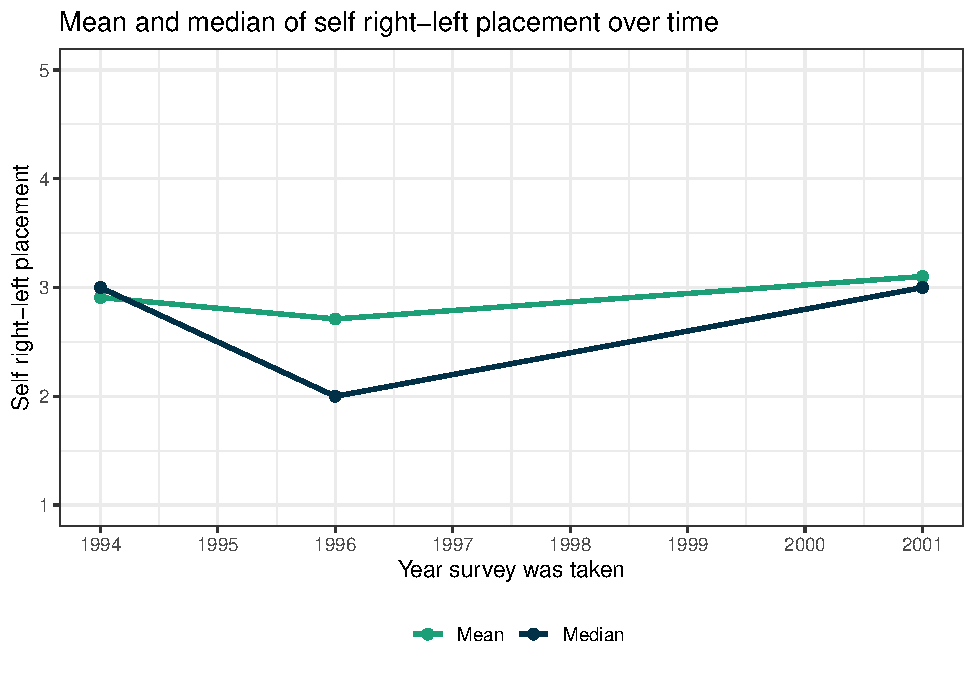
\includegraphics{AVCD-Assignment2-Edenhofer_files/figure-latex/mean-self-rl-over-time-1.pdf}

We can see that, in 1994 and 2001, the mean and median are both roughly
three, suggesting that in these two years the distribution of
ideological self-placement is roughly normal. In 1996, however, the mean
is higher than the median, i.e.~the median has ideologically shifted to
the right. Because of the labelling of \texttt{place\_self} (1 == right,
5 == left), the distribution of \texttt{place\_self} in that election
year is, in statistical language, skewed to the left, which,
substantively, is due to an increase in the share of fairly extreme
right-wing respondents in that year.

Without taking into account the variance or standard deviation of the
mean of \texttt{place\_self}, we cannot determine whether the
ideological right-ward shift in 1996 is a statistically significant one.
To that end, I run the following code:

\begin{Shaded}
\begin{Highlighting}[]
\NormalTok{deV07\_mod }\SpecialCharTok{\%\textgreater{}\%}
  \FunctionTok{group\_by}\NormalTok{(year) }\SpecialCharTok{\%\textgreater{}\%}
  \FunctionTok{summarise}\NormalTok{(}\FunctionTok{round}\NormalTok{(}\FunctionTok{mean\_cl\_normal}\NormalTok{(place\_self), }\AttributeTok{digits =} \DecValTok{2}\NormalTok{)) }\SpecialCharTok{\%\textgreater{}\%}
  \FunctionTok{kbl}\NormalTok{(}\AttributeTok{booktabs =}\NormalTok{ T, }
      \AttributeTok{col.names =} \FunctionTok{c}\NormalTok{(}\StringTok{"Year"}\NormalTok{, }\StringTok{"Mean"}\NormalTok{, }\StringTok{"Lower bound of 95\% CI"}\NormalTok{,}
                      \StringTok{"Upper bound of 95\% CI"}\NormalTok{), }
      \AttributeTok{caption =} \StringTok{"Mean of ideological shift"}\NormalTok{) }\SpecialCharTok{\%\textgreater{}\%}
  \FunctionTok{kable\_styling}\NormalTok{(}\AttributeTok{latex\_options =} \StringTok{"hold\_position"}\NormalTok{)}
\end{Highlighting}
\end{Shaded}

\begin{table}[!h]

\caption{\label{tab:ideo-shift-table}Mean of ideological shift}
\centering
\begin{tabular}[t]{rrrr}
\toprule
Year & Mean & Lower bound of 95\% CI & Upper bound of 95\% CI\\
\midrule
1994 & 2.91 & 2.81 & 3.01\\
1996 & 2.71 & 2.65 & 2.77\\
2001 & 3.10 & 3.03 & 3.17\\
\bottomrule
\end{tabular}
\end{table}

Since the lower bound of the 1994 mean value is greater than the upper
bound for the 1996 mean value, we can conclude\footnote{Non-overlapping
  confidence intervals imply significance, while the overlapping ones do
  not allow us to make any inferences about significance
  (\protect\hyperlink{ref-gailmard_statistical_2014}{Gailmard 2014}).}
that the ideological right-ward shift is statistically significant at
the 5\% level. The overall conclusion is then that there is a
significant right-ward shift from the 1994 to 1996 survey, which,
however, is fully reversed by 2001.

\textcolor{brown}{Following De Vries (2007), measure the perceived distance betwen voters and their party of choice. Why would do you square it? And what is the main implication for results interpretation?}

To create the desired variable, I subtract \texttt{place\_self} from
\texttt{place\_votedprty} and then square that difference.

\begin{Shaded}
\begin{Highlighting}[]
\NormalTok{deV07\_mod }\OtherTok{\textless{}{-}}\NormalTok{ deV07\_mod }\SpecialCharTok{\%\textgreater{}\%}
  \FunctionTok{mutate}\NormalTok{(}\AttributeTok{squared\_distance =}\NormalTok{ (place\_self}\SpecialCharTok{{-}}\NormalTok{place\_votedprty)}\SpecialCharTok{\^{}}\DecValTok{2}\NormalTok{)  }
\end{Highlighting}
\end{Shaded}

The resulting difference is referred to as the \emph{Euclidean}
distance, which is minimised when the voter's self-placement equals the
party's ideological position, as perceived by that voter. Consequently,
increases in the Euclidean distance indicate increases in the perceived
ideological distance between a voter-party pair, with the square
ensuring that (i) left and right differences are treated identically,
and (ii) that greater deviations are weighted more heavily, i.e.~the
possible differences are 0, 1, 4, 9, and 16.

\hypertarget{section-2}{%
\subsection{1.3}\label{section-2}}

\textcolor{brown}{What pushes individuals to vote for parties with extreme right-left placements? Estimate the appropriate model and report it a nice, tidy table. Explain why you controlled for the covariates that you picked.What model did you use in the previous point? Why? Plot the coefficients and comment their magnitude and level of statistical significance}

My dependent variable is the \texttt{extreme\_dummy\_parties} variable
created in 1.1, which is unity of voters perceive a party as either
extreme right or left wing. To identify the correlates of extreme
voting, I run six models.

\begin{itemize}
\item
  In the first model, I simply regress the dependent variable on
  \texttt{squared\_distance}. This is motivated by the spatial theory of
  voting, which predicts that individuals will vote for those parties
  that they perceive to be ideologically closest to them. Hence, I
  expect the coefficient estimate to be \emph{negative} since increases
  \texttt{squared\_distance} mean lower ideological proximity, as
  explained in 1.2.
\item
  In the second model, I add the \texttt{gndr\_dummy}. This is motivated
  by recent findings (e.g.
  \protect\hyperlink{ref-anduiza2022sexism}{Anduiza and Rico 2022};
  \protect\hyperlink{ref-oshri2022risk}{Oshri et al. 2022}) that men
  are, ceteris paribus, more likely than women to vote for radical right
  parties. Therefore, I expect the coefficient estimate to be
  \emph{positive}\footnote{The dummy variable, recall, is unity for men
    and zero otherwise.}, though this is more of a tentative hypothesis.
  This is because the dependent variable also includes radical left
  parties and the theoretical expectations are less clear for that party
  family.
\item
  The third model adds education, which is widely considered to be one
  of the most powerful predictors of vote choice. Given that higher
  values indicate greater education, I expect the coefficient estimate
  to be \emph{negative}.
\item
  The fourth model adds religiosity, reflecting theoretical arguments
  relating religiosity to extreme voting. Some argue that greater
  religiosity decreases the probability of voting for an extreme party
  by creating a strong attachment to religious parties, notably the
  Christian democrats
  (\protect\hyperlink{ref-arzheimer2009christian}{Arzheimer and Carter
  2009}). Others contend that religiosity can push individuals to the
  extreme right on account of promoting social conservatism
  (\protect\hyperlink{ref-marcinkiewicz2022religious}{Marcinkiewicz and
  Dassonneville 2022}). Hence, the sign is theoretically indeterminate.
\item
  The fifth model adds the salience of unemployment in a given election
  year, with greater salience potentially pushing voters towards the
  extremes (\emph{positive} coefficient estimate). On the other hand,
  voters may care more about competence in economically hard times, and
  elect moderate parties, provided, of course, that they believe these
  parties to be more competent.
\item
  The sixth model adds a proxy for political interest. Given the coding
  of the variable, I expect a \emph{positive} coefficient estimate,
  indicating that less interested individuals are more likely to vote
  for extreme parties, holding all other included variables constant.
\end{itemize}

\begin{Shaded}
\begin{Highlighting}[]
\NormalTok{extreme\_party1 }\OtherTok{\textless{}{-}} \FunctionTok{glm}\NormalTok{(extreme\_dummy\_parties }\SpecialCharTok{\textasciitilde{}}\NormalTok{ squared\_distance, }
                     \AttributeTok{family =} \FunctionTok{binomial}\NormalTok{(}\AttributeTok{link =} \StringTok{"logit"}\NormalTok{),}
                     \AttributeTok{data =}\NormalTok{ deV07\_mod)}
\NormalTok{extreme\_party2 }\OtherTok{\textless{}{-}} \FunctionTok{glm}\NormalTok{(extreme\_dummy\_parties }\SpecialCharTok{\textasciitilde{}}\NormalTok{ squared\_distance }\SpecialCharTok{+}\NormalTok{ gndr\_dummy, }
                     \AttributeTok{family =} \FunctionTok{binomial}\NormalTok{(}\AttributeTok{link =} \StringTok{"logit"}\NormalTok{),}
                     \AttributeTok{data =}\NormalTok{ deV07\_mod)}
\NormalTok{extreme\_party3 }\OtherTok{\textless{}{-}} \FunctionTok{glm}\NormalTok{(extreme\_dummy\_parties }\SpecialCharTok{\textasciitilde{}}\NormalTok{ squared\_distance }\SpecialCharTok{+}\NormalTok{ gndr\_dummy }\SpecialCharTok{+}\NormalTok{ edu, }
                     \AttributeTok{family =} \FunctionTok{binomial}\NormalTok{(}\AttributeTok{link =} \StringTok{"logit"}\NormalTok{),}
                     \AttributeTok{data =}\NormalTok{ deV07\_mod)}
\NormalTok{extreme\_party4 }\OtherTok{\textless{}{-}} \FunctionTok{glm}\NormalTok{(extreme\_dummy\_parties }\SpecialCharTok{\textasciitilde{}}\NormalTok{ squared\_distance }\SpecialCharTok{+}\NormalTok{ gndr\_dummy }\SpecialCharTok{+}\NormalTok{ edu }\SpecialCharTok{+}\NormalTok{ relig, }
                     \AttributeTok{family =} \FunctionTok{binomial}\NormalTok{(}\AttributeTok{link =} \StringTok{"logit"}\NormalTok{),}
                     \AttributeTok{data =}\NormalTok{ deV07\_mod)}
\NormalTok{extreme\_party5 }\OtherTok{\textless{}{-}} \FunctionTok{glm}\NormalTok{(extreme\_dummy\_parties }\SpecialCharTok{\textasciitilde{}}\NormalTok{ squared\_distance }\SpecialCharTok{+}\NormalTok{ gndr\_dummy }\SpecialCharTok{+}\NormalTok{ edu }\SpecialCharTok{+}\NormalTok{ relig }\SpecialCharTok{+}\NormalTok{ unemp\_salience\_per\_year, }
                     \AttributeTok{family =} \FunctionTok{binomial}\NormalTok{(}\AttributeTok{link =} \StringTok{"logit"}\NormalTok{),}
                     \AttributeTok{data =}\NormalTok{ deV07\_mod)}
\NormalTok{extreme\_party6 }\OtherTok{\textless{}{-}} \FunctionTok{glm}\NormalTok{(extreme\_dummy\_parties }\SpecialCharTok{\textasciitilde{}}\NormalTok{ squared\_distance }\SpecialCharTok{+}\NormalTok{ gndr\_dummy }\SpecialCharTok{+}\NormalTok{ edu }\SpecialCharTok{+}\NormalTok{ relig }\SpecialCharTok{+}\NormalTok{ unemp\_salience\_per\_year }\SpecialCharTok{+}\NormalTok{ debate, }
                     \AttributeTok{family =} \FunctionTok{binomial}\NormalTok{(}\AttributeTok{link =} \StringTok{"logit"}\NormalTok{),}
                     \AttributeTok{data =}\NormalTok{ deV07\_mod)}
\CommentTok{\# modelsummary }
\FunctionTok{modelsummary}\NormalTok{(}\FunctionTok{list}\NormalTok{(extreme\_party1, extreme\_party2, extreme\_party3, extreme\_party4, extreme\_party5, extreme\_party6), }
             \AttributeTok{estimate =} \StringTok{"\{estimate\}\{stars\}"}\NormalTok{, }
             \AttributeTok{coef\_map =} \FunctionTok{c}\NormalTok{(}\StringTok{"squared\_distance"} \OtherTok{=} \StringTok{"Perceived squared distance"}\NormalTok{, }
                          \StringTok{"gndr\_dummy"} \OtherTok{=} \StringTok{"Gender dummy"}\NormalTok{, }
                          \StringTok{"edu"} \OtherTok{=} \StringTok{"Education"}\NormalTok{, }
                          \StringTok{"relig"} \OtherTok{=} \StringTok{"Religiosity"}\NormalTok{, }
                          \StringTok{"unemp\_salience\_per\_year"} \OtherTok{=} \StringTok{"Salience of unemployment"}\NormalTok{,}
                          \StringTok{"debate"} \OtherTok{=} \StringTok{"Political interest"}\NormalTok{),}
             \AttributeTok{title =} \StringTok{"Correlates of extreme voting"}\NormalTok{) }\SpecialCharTok{\%\textgreater{}\%}
  \FunctionTok{kable\_styling}\NormalTok{(}\AttributeTok{latex\_options =} \StringTok{"hold\_position"}\NormalTok{)}
\end{Highlighting}
\end{Shaded}

\begin{table}[!h]

\caption{\label{tab:extreme-party-model}Correlates of extreme voting}
\centering
\begin{tabular}[t]{lcccccc}
\toprule
  & (1) & (2) & (3) & (4) & (5) & (6)\\
\midrule
Perceived squared distance & \num{0.106}*** & \num{0.105}*** & \num{0.127}*** & \num{0.137}*** & \num{0.190}*** & \num{0.215}***\\
 & (\num{0.014}) & (\num{0.014}) & (\num{0.015}) & (\num{0.015}) & (\num{0.017}) & (\num{0.018})\\
Gender dummy &  & \num{-0.084} & \num{-0.071} & \num{-0.085} & \num{-0.087} & \num{-0.018}\\
 &  & (\num{0.082}) & (\num{0.084}) & (\num{0.087}) & (\num{0.089}) & (\num{0.091})\\
Education &  &  & \num{-0.330}*** & \num{-0.338}*** & \num{-0.250}*** & \num{-0.179}***\\
 &  &  & (\num{0.028}) & (\num{0.028}) & (\num{0.030}) & (\num{0.032})\\
Religiosity &  &  &  & \num{-0.004} & \num{-0.030} & \num{-0.015}\\
 &  &  &  & (\num{0.035}) & (\num{0.036}) & (\num{0.037})\\
Salience of unemployment &  &  &  &  & \num{-2.324}*** & \num{-2.759}***\\
 &  &  &  &  & (\num{0.223}) & (\num{0.242})\\
Political interest &  &  &  &  &  & \num{0.494}***\\
 &  &  &  &  &  & (\num{0.056})\\
\midrule
Num.Obs. & \num{3050} & \num{3050} & \num{3049} & \num{2952} & \num{2952} & \num{2951}\\
AIC & \num{3610.4} & \num{3611.4} & \num{3463.0} & \num{3301.1} & \num{3193.3} & \num{3112.7}\\
BIC & \num{3622.5} & \num{3629.5} & \num{3487.1} & \num{3331.1} & \num{3229.3} & \num{3154.6}\\
Log.Lik. & \num{-1803.224} & \num{-1802.697} & \num{-1727.509} & \num{-1645.564} & \num{-1590.667} & \num{-1549.336}\\
F & \num{55.684} & \num{28.351} & \num{62.673} & \num{48.398} & \num{54.552} & \num{51.648}\\
RMSE & \num{0.45} & \num{0.45} & \num{0.44} & \num{0.43} & \num{0.43} & \num{0.42}\\
\bottomrule
\end{tabular}
\end{table}

To represent the results in a coefficient plot, I use the
\texttt{modelplot()} function because the latter can be more easily
integrated with the \texttt{kableExtra} package than the
\texttt{coefplot()} function.

\begin{Shaded}
\begin{Highlighting}[]
\FunctionTok{modelplot}\NormalTok{(}\FunctionTok{list}\NormalTok{(extreme\_party1, extreme\_party2, extreme\_party3, extreme\_party4, extreme\_party5, extreme\_party6),}
         \AttributeTok{coef\_map =} \FunctionTok{c}\NormalTok{(}\StringTok{"squared\_distance"} \OtherTok{=} \StringTok{"Perceived squared distance"}\NormalTok{, }
                      \StringTok{"gndr\_dummy"} \OtherTok{=} \StringTok{"Gender dummy"}\NormalTok{, }
                      \StringTok{"edu"} \OtherTok{=} \StringTok{"Education"}\NormalTok{, }
                      \StringTok{"relig"} \OtherTok{=} \StringTok{"Religiosity"}\NormalTok{, }
                      \StringTok{"debate"} \OtherTok{=} \StringTok{"Political interest"}\NormalTok{,}
                      \StringTok{"unemp\_salience\_per\_year"} \OtherTok{=} \StringTok{"Salience of unemployment"}\NormalTok{)) }\SpecialCharTok{+}
  \FunctionTok{expand\_limits}\NormalTok{(}\AttributeTok{x =} \DecValTok{1}\NormalTok{) }\SpecialCharTok{+}
  \FunctionTok{geom\_vline}\NormalTok{(}\AttributeTok{xintercept =} \DecValTok{0}\NormalTok{, }\AttributeTok{linetype =} \StringTok{"dashed"}\NormalTok{) }\SpecialCharTok{+}
  \FunctionTok{labs}\NormalTok{(}\AttributeTok{title =} \StringTok{"Coefficient plot of the six models"}\NormalTok{) }\SpecialCharTok{+}
  \FunctionTok{theme}\NormalTok{(}\AttributeTok{legend.position =} \StringTok{"bottom"}\NormalTok{)}
\end{Highlighting}
\end{Shaded}

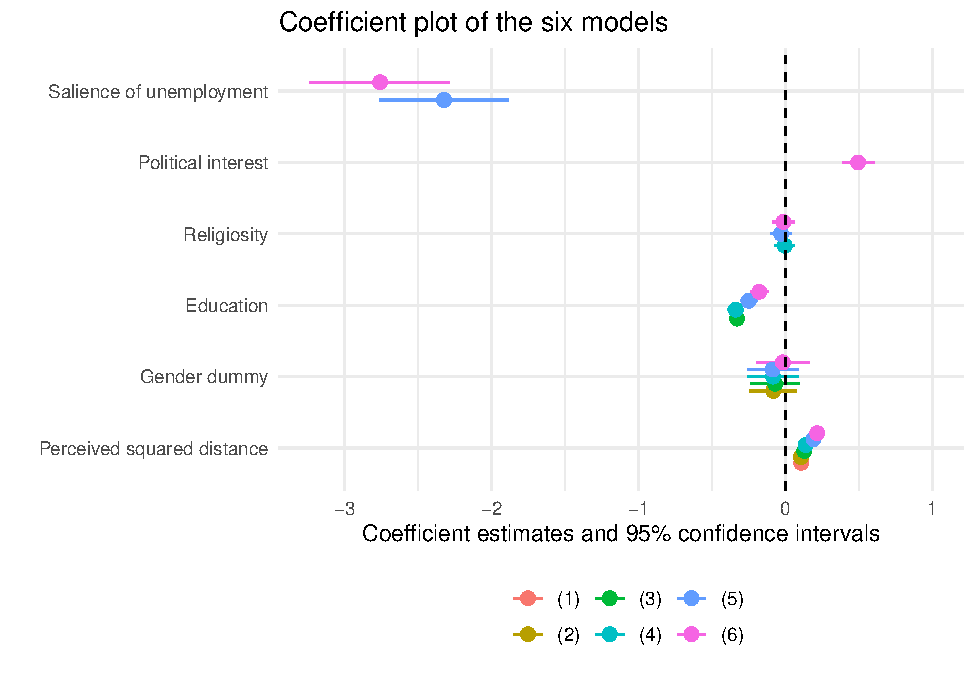
\includegraphics{AVCD-Assignment2-Edenhofer_files/figure-latex/coefplots-extreme-choice-1.pdf}

The above plot and table 3 reveal four significant correlates of extreme
voting:

\begin{itemize}
\item
  The \texttt{squared\_distance} term is significant, but the sign is
  the opposite of what spatial voting theory would lead us to expect.
  That is, as the squared distance increases by one unit (i.e.~as there
  is less ideological proximity), the probability of extreme voting
  increases. Specifically, the log odds increase by roughly 24\%
  (\(100*(exp(0.215)-1)\)), holding all other included covariates
  constant.
\item
  Greater levels of education are, as expected, significantly associated
  with a lower probability of extreme voting, with the log odds
  decreasing by roughly 16.4\% (\(100*(exp(-0.179)-1)\)) for a unit
  increase in the level of education.
\item
  As the share of voters that regard unemployment as the most important
  issue rises, the probability of extreme voting decreases significantly
  - the log odds increase by approximately 95\%
  (\(100*(exp(-2.759)-1)\)). Put simply: there is a strong inverse
  association between the salience of unemployment and extreme voting.
  This is consistent with the ``competence'' mechanism outlined above,
  though the results should not be interpreted as direct evidence for
  that mechanism.
\item
  As expected, less politically interested voters are, ceteris paribus,
  more likely to vote for extreme parties, with the log odds increasing
  by roughly 64\% (\(100*(exp(0.494)-1)\)) for a unit increase in
  political interest.
\end{itemize}

\hypertarget{exercise-2}{%
\section{Exercise 2}\label{exercise-2}}

\hypertarget{section-3}{%
\subsection{2.1}\label{section-3}}

\textcolor{brown}{What is the effect of gender on interest for politics (measured as watching TV debate)? Does it change when individuals are very concerned by unemployment? If so, how? Write down the formal models you have estimated, explain what the coefficients represent, and interpret the results.}

To examine the relationship of interest, I begin by dichotomising the
\texttt{debate} variable such that it is unity when a respondent watches
TV debates at all and zero otherwise. I then regress this variable on
the gender dummy in the first model, and add an interaction term between
the latter and the unemployment issue dummy in the second model. The
interaction terms allows us to examine whether the effect of gender on
political interest varies by the importance respondents attach to
unemployment as a political issue. In the third model, I add education
and religiosity as covariates to probe the robustness of the results
obtained from the previous models. My estimating equation for this final
model is:

\[
\begin{aligned}
log(\frac{Interest_{i}}{1-Interest_{i}}) = \alpha + \beta_{1}Gender_{i} +  \beta_{2}Unemployment_{i} + \beta_{3}Gender_{i}*Unemployment_{i} \\ 
+ \beta_{4}Education_{i} + \beta_{5}Religiosity_{i} + \epsilon_{i}
\end{aligned}
\]

In R, I estimate this equation by running:

\begin{Shaded}
\begin{Highlighting}[]
\CommentTok{\# create dummy variable }
\NormalTok{deV07\_mod }\OtherTok{\textless{}{-}}\NormalTok{ deV07\_mod }\SpecialCharTok{\%\textgreater{}\%}
  \FunctionTok{mutate}\NormalTok{(}\AttributeTok{interest\_dummy =} \FunctionTok{ifelse}\NormalTok{(debate }\SpecialCharTok{\%in\%} \FunctionTok{c}\NormalTok{(}\DecValTok{1}\NormalTok{, }\DecValTok{2}\NormalTok{), }\DecValTok{1}\NormalTok{, }\DecValTok{0}\NormalTok{),}
         \CommentTok{\# factorise to increase interpretability}
         \AttributeTok{gndr\_dummy\_f =} \FunctionTok{factor}\NormalTok{(gndr\_dummy, }
                               \AttributeTok{levels =} \FunctionTok{c}\NormalTok{(}\StringTok{"0"}\NormalTok{, }\StringTok{"1"}\NormalTok{), }
                               \AttributeTok{labels =} \FunctionTok{c}\NormalTok{(}\StringTok{"Female"}\NormalTok{, }\StringTok{"Male"}\NormalTok{)), }
         \AttributeTok{unemp\_issue\_f =} \FunctionTok{factor}\NormalTok{(unemp\_issue,}
                               \AttributeTok{levels =} \FunctionTok{c}\NormalTok{(}\StringTok{"0"}\NormalTok{, }\StringTok{"1"}\NormalTok{), }
                               \AttributeTok{labels =} \FunctionTok{c}\NormalTok{(}\StringTok{"No"}\NormalTok{, }\StringTok{"Yes"}\NormalTok{)))}

\CommentTok{\# estimate logit model }
\NormalTok{interest1 }\OtherTok{\textless{}{-}} \FunctionTok{glm}\NormalTok{(interest\_dummy }\SpecialCharTok{\textasciitilde{}}\NormalTok{ gndr\_dummy\_f, }
                 \AttributeTok{family =} \FunctionTok{binomial}\NormalTok{(}\AttributeTok{link =} \StringTok{"logit"}\NormalTok{), }
                 \AttributeTok{data =}\NormalTok{ deV07\_mod)}
\NormalTok{interest2 }\OtherTok{\textless{}{-}} \FunctionTok{glm}\NormalTok{(interest\_dummy }\SpecialCharTok{\textasciitilde{}}\NormalTok{ gndr\_dummy\_f}\SpecialCharTok{*}\NormalTok{unemp\_issue\_f, }
                 \AttributeTok{family =} \FunctionTok{binomial}\NormalTok{(}\AttributeTok{link =} \StringTok{"logit"}\NormalTok{), }
                 \AttributeTok{data =}\NormalTok{ deV07\_mod)}
\NormalTok{interest3 }\OtherTok{\textless{}{-}} \FunctionTok{glm}\NormalTok{(interest\_dummy }\SpecialCharTok{\textasciitilde{}}\NormalTok{ gndr\_dummy\_f}\SpecialCharTok{*}\NormalTok{unemp\_issue\_f }\SpecialCharTok{+}\NormalTok{ edu }\SpecialCharTok{+}\NormalTok{ relig, }
                 \AttributeTok{family =} \FunctionTok{binomial}\NormalTok{(}\AttributeTok{link =} \StringTok{"logit"}\NormalTok{), }
                 \AttributeTok{data =}\NormalTok{ deV07\_mod)}

\CommentTok{\# modelsummary }
\FunctionTok{modelsummary}\NormalTok{(}\FunctionTok{list}\NormalTok{(interest1, interest2, interest3), }
             \AttributeTok{estimate =} \StringTok{"\{estimate\}\{stars\}"}\NormalTok{,}
             \AttributeTok{coef\_map =} \FunctionTok{c}\NormalTok{(}\StringTok{"gndr\_dummy\_fMale"} \OtherTok{=} \StringTok{"Gender"}\NormalTok{, }
                          \StringTok{"unemp\_issue\_f1"} \OtherTok{=} \StringTok{"Unemployment most important issue"}\NormalTok{, }
                          \StringTok{"gndr\_dummy\_fMale:unemp\_issue\_f1"} \OtherTok{=} \StringTok{"Gender x Unemployment most important issue"}\NormalTok{,}
                          \StringTok{"edu"} \OtherTok{=} \StringTok{"Education"}\NormalTok{, }
                          \StringTok{"relig"} \OtherTok{=} \StringTok{"Religiosity"}\NormalTok{), }
             \AttributeTok{title =} \StringTok{"Association between interest in politics and gender"}\NormalTok{) }\SpecialCharTok{\%\textgreater{}\%}
  \FunctionTok{kable\_styling}\NormalTok{(}\AttributeTok{latex\_options =} \StringTok{"hold\_position"}\NormalTok{)}
\end{Highlighting}
\end{Shaded}

\begin{table}[!h]

\caption{\label{tab:gender-interest-relation}Association between interest in politics and gender}
\centering
\begin{tabular}[t]{lccc}
\toprule
  & (1) & (2) & (3)\\
\midrule
Gender & \num{0.231}*** & \num{0.212}* & \num{0.297}**\\
 & (\num{0.067}) & (\num{0.098}) & (\num{0.111})\\
Education &  &  & \num{0.652}***\\
 &  &  & (\num{0.029})\\
Religiosity &  &  & \num{0.125}***\\
 &  &  & (\num{0.034})\\
\midrule
Num.Obs. & \num{4091} & \num{3299} & \num{3278}\\
AIC & \num{5200.5} & \num{4319.0} & \num{3665.7}\\
BIC & \num{5213.1} & \num{4343.4} & \num{3702.2}\\
Log.Lik. & \num{-2598.229} & \num{-2155.511} & \num{-1826.836}\\
F & \num{11.971} & \num{31.815} & \num{112.216}\\
RMSE & \num{0.47} & \num{0.48} & \num{0.44}\\
\bottomrule
\end{tabular}
\end{table}

To interpret the coefficient estimates, it is worth writing out the
conditional expectations the above regression implies. To that end, let
us define \(\phi\) as a shorthand for
\(log(\frac{Interest_{i}}{1-Interest_{i}})\), and let \(\hat{Educ}\) and
\(\hat{Relig}\) denote fixed values of these covariates. Then, we can
write:

\[
\begin{aligned}
\mathbb{E}[\phi \vert Gender_{i} = 0, Unemployment_{i} = 0, \hat{Educ_{i}}, \hat{Relig_{i}}] = \alpha + \beta_{4}\hat{Educ_{i}} + \beta_{5}\hat{Relig_{i}} \\
\mathbb{E}[\phi \vert Gender_{i} = 1, Unemployment_{i} = 0, \hat{Educ_{i}}, \hat{Relig_{i}}] = \alpha + \beta_{1} + \beta_{4}\hat{Educ_{i}} + \beta_{5}\hat{Relig_{i}} \\
\mathbb{E}[\phi \vert Gender_{i} = 0, Unemployment_{i} = 1, \hat{Educ_{i}}, \hat{Relig_{i}}] = \alpha + \beta_{2} + \beta_{4}\hat{Educ_{i}} + \beta_{5}\hat{Relig_{i}} \\
\mathbb{E}[\phi \vert Gender_{i} = 1, Unemployment_{i} = 1, \hat{Educ_{i}}, \hat{Relig_{i}}] = \alpha + \beta_{1} + \beta_{2} + \beta_{3} + \beta_{4}\hat{Educ_{i}} + \beta_{5}\hat{Relig_{i}} \\
\end{aligned}
\]

Subtracting the first equation from the second gives us \(\beta_{1}\).
Substantively, \(\beta_{1}\) therefore represents the marginal effect of
gender on political interest, i.e.~the change in the expected
probability of watching TV debates for males (gender = 1) compared to
females (gender = 0), holding the values of education and religiosity
constant. Similarly, subtracting the third equation from the first gives
us \(\beta_{2}\). Hence, \(\beta_{2}\) represents the marginal effect of
unemployment importance on political interest, i.e.~the change in the
expected probability of watching TV debates for those viewing
unemployment as the most important political issue, compared to those
who do not do so, holding the values of education and religiosity
constant. Finally, the coefficient on the interaction term is obtained
by subtracting (i) equation three from four, (ii) subtracting one from
two, and (iii) subtracting the second difference from the first.
Intuitively, this means that the interaction term represents the
difference in the marginal effect of gender between those who view
unemployment as the most important issue, compared to those who do not,
holding all other covariates constant.

Table 4 allows us to draw four lessons:

\begin{itemize}
\item
  Males exhibit significantly greater political interest than females,
  holding all other included covariates constant, with the log odds of
  watching TV debates being approximately 34.6\%
  (\(100*(exp(0.297)-1)\)) higher for males than females.
\item
  Similarly, those considering unemployment the most important political
  issue exhibit, ceteris paribus, greater political interest than those
  who do consider unemployment as important, with the log odds being
  being 74\% (\(100*(exp(0.554)-1)\)) higher for the former, compared to
  the latter.
\item
  The marginal effect of gender on political interest does not
  significantly vary with the unemployment dummy, as the coefficient
  estimate in the third row shows.
\item
  Both greater religiosity and higher education levels are positively
  and significantly associated with political interest.
\end{itemize}

\hypertarget{section-4}{%
\subsection{2.2}\label{section-4}}

\textcolor{brown}{Represent graphically: The predicted probabilities of gender on interest in politics when unemployment is the most important issue (or not), The marginal effects of gender on interest in politics when unemployment is the most important issue (or not), Put the two graphs in a singular imagine}

To plot the predicted probabilities, I use the \texttt{ggeffects}
package. The plot below includes connecting lines as visual aids for
tracking how the effect of gender varies across unemployment.

\begin{Shaded}
\begin{Highlighting}[]
\NormalTok{pp\_plot }\OtherTok{\textless{}{-}} \FunctionTok{plot}\NormalTok{(}\FunctionTok{ggpredict}\NormalTok{(interest3, }\AttributeTok{terms =} \FunctionTok{c}\NormalTok{(}\StringTok{"unemp\_issue\_f"}\NormalTok{, }\StringTok{"gndr\_dummy\_f"}\NormalTok{)), }
     \AttributeTok{connect.lines =}\NormalTok{ T) }\SpecialCharTok{+}
  \FunctionTok{scale\_colour\_manual}\NormalTok{(}\StringTok{"Gender"}\NormalTok{,}
                      \AttributeTok{labels =} \FunctionTok{c}\NormalTok{(}\StringTok{"0"} \OtherTok{=} \StringTok{"Female"}\NormalTok{,}
                                 \StringTok{"1"} \OtherTok{=} \StringTok{"Male"}\NormalTok{),}
                      \AttributeTok{values =} \FunctionTok{c}\NormalTok{(}\FunctionTok{c}\NormalTok{(}\StringTok{"\#1C9E77"}\NormalTok{, }\StringTok{"\#023047"}\NormalTok{))) }\SpecialCharTok{+}
  \FunctionTok{expand\_limits}\NormalTok{(}\AttributeTok{y =} \FloatTok{0.8}\NormalTok{) }\SpecialCharTok{+}
  \FunctionTok{labs}\NormalTok{(}\AttributeTok{y =} \StringTok{"Predicted probability of watching debates"}\NormalTok{,}
       \AttributeTok{x =} \StringTok{"Unemployment most important issue?"}\NormalTok{,}
       \AttributeTok{title =} \StringTok{"Predicted probabilities}\SpecialCharTok{\textbackslash{}n}\StringTok{of being interested in politics"}\NormalTok{, }
       \AttributeTok{caption =} \StringTok{"Covariates include: education and religiosity."}\NormalTok{) }\SpecialCharTok{+}
  \FunctionTok{theme}\NormalTok{(}\AttributeTok{legend.position =} \StringTok{"bottom"}\NormalTok{) }\SpecialCharTok{+}
  \FunctionTok{theme}\NormalTok{(}\AttributeTok{plot.title =} \FunctionTok{element\_text}\NormalTok{(}\AttributeTok{size =} \DecValTok{10}\NormalTok{),}
        \AttributeTok{plot.caption =} \FunctionTok{element\_text}\NormalTok{(}\AttributeTok{hjust =} \DecValTok{0}\NormalTok{, }\AttributeTok{size =} \DecValTok{6}\NormalTok{))}
\end{Highlighting}
\end{Shaded}

To compute the marginal effect, I use the \texttt{cplot()} from the
\texttt{margins} package.

\begin{Shaded}
\begin{Highlighting}[]
\CommentTok{\# compute marginal effect}
\NormalTok{interest4 }\OtherTok{\textless{}{-}} \FunctionTok{glm}\NormalTok{(interest\_dummy }\SpecialCharTok{\textasciitilde{}}\NormalTok{ gndr\_dummy}\SpecialCharTok{*}\NormalTok{unemp\_issue\_f }\SpecialCharTok{+}\NormalTok{ edu }\SpecialCharTok{+}\NormalTok{ relig, }
                 \AttributeTok{family =} \FunctionTok{binomial}\NormalTok{(}\AttributeTok{link =} \StringTok{"logit"}\NormalTok{), }
                 \AttributeTok{data =}\NormalTok{ deV07\_mod)}
\NormalTok{me }\OtherTok{\textless{}{-}}\NormalTok{ margins}\SpecialCharTok{::}\FunctionTok{cplot}\NormalTok{(interest4, }\AttributeTok{dx =} \StringTok{"gndr\_dummy"}\NormalTok{, }
               \AttributeTok{x =} \StringTok{"unemp\_issue\_f"}\NormalTok{, }\AttributeTok{what =} \StringTok{"effect"}\NormalTok{, }\AttributeTok{draw =}\NormalTok{ F)}
\CommentTok{\# marginal effect plot }
\NormalTok{me\_plot }\OtherTok{\textless{}{-}}\NormalTok{ me }\SpecialCharTok{\%\textgreater{}\%}
  \FunctionTok{ggplot}\NormalTok{(}\FunctionTok{aes}\NormalTok{(}\AttributeTok{x =}\NormalTok{ xvals, }\AttributeTok{y =}\NormalTok{ yvals)) }\SpecialCharTok{+}
  \FunctionTok{geom\_point}\NormalTok{(}\AttributeTok{size =} \DecValTok{2}\NormalTok{) }\SpecialCharTok{+}
  \FunctionTok{geom\_errorbar}\NormalTok{(}\FunctionTok{aes}\NormalTok{(}\AttributeTok{ymin =}\NormalTok{ lower, }\AttributeTok{ymax =}\NormalTok{ upper), }\AttributeTok{width =} \FloatTok{0.2}\NormalTok{) }\SpecialCharTok{+}
  \FunctionTok{geom\_hline}\NormalTok{(}\AttributeTok{yintercept =} \DecValTok{0}\NormalTok{, }\AttributeTok{linetype =} \StringTok{"dashed"}\NormalTok{) }\SpecialCharTok{+}
  \FunctionTok{expand\_limits}\NormalTok{(}\AttributeTok{y =} \FloatTok{0.12}\NormalTok{) }\SpecialCharTok{+}
  \FunctionTok{labs}\NormalTok{(}\AttributeTok{y =} \StringTok{"Marginal effect"}\NormalTok{, }
       \AttributeTok{x =} \StringTok{"Unemployment most important issue?"}\NormalTok{,}
       \AttributeTok{title =} \StringTok{"Marginal effect of gender on}\SpecialCharTok{\textbackslash{}n}\StringTok{political interest by unemployment salience"}\NormalTok{,}
       \AttributeTok{caption =} \StringTok{"Covariates include: education and religiosity."}\NormalTok{) }\SpecialCharTok{+}
  \FunctionTok{theme\_bw}\NormalTok{() }\SpecialCharTok{+}
  \FunctionTok{theme}\NormalTok{(}\AttributeTok{plot.title =} \FunctionTok{element\_text}\NormalTok{(}\AttributeTok{size =} \DecValTok{10}\NormalTok{),}
        \AttributeTok{plot.caption =} \FunctionTok{element\_text}\NormalTok{(}\AttributeTok{hjust =} \DecValTok{0}\NormalTok{, }\AttributeTok{size =} \DecValTok{6}\NormalTok{))}
\end{Highlighting}
\end{Shaded}

I combine the two plots using the \texttt{ggarrange()} function.

\begin{Shaded}
\begin{Highlighting}[]
\FunctionTok{ggarrange}\NormalTok{(pp\_plot, me\_plot, }\AttributeTok{nrow =} \DecValTok{1}\NormalTok{)}
\end{Highlighting}
\end{Shaded}

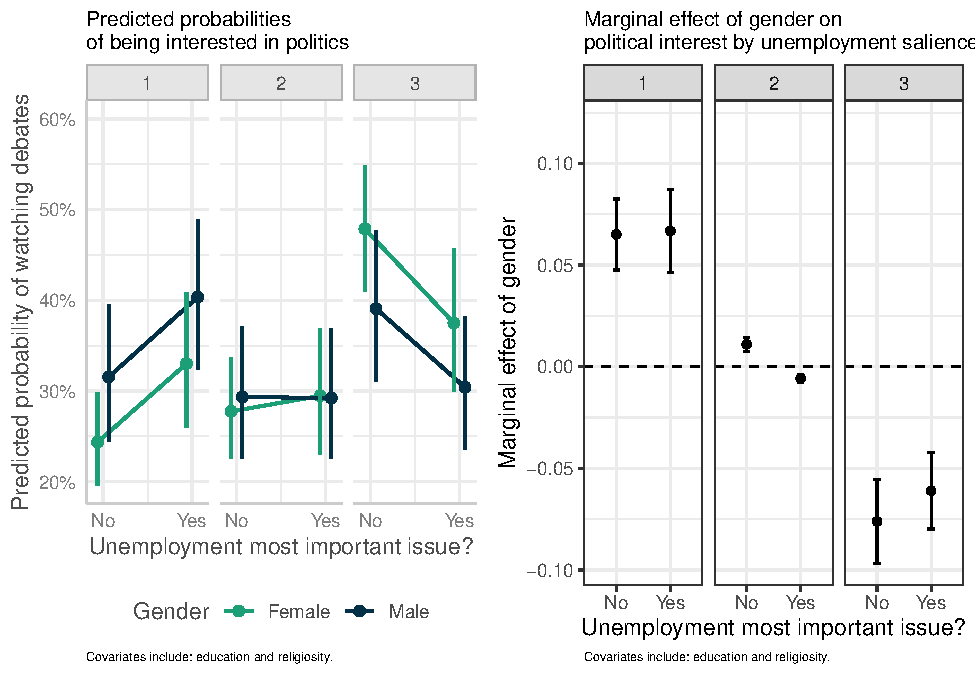
\includegraphics{AVCD-Assignment2-Edenhofer_files/figure-latex/pp-and-me-combined-1.pdf}

As explained above, the marginal effect of gender is the vertical
difference in predicted probabilities for males and females
respectively. Analogously, the marginal effect of unemployment is the
horizontal difference between the blue and green point estimates
respectively. The two horizontal differences are almost identical. This,
in combination with the almost completely overlapping confidence
intervals for the marginal effects, confirms our conclusion that the
effect of gender does not change significantly with unemployment.

\hypertarget{section-5}{%
\subsection{2.3}\label{section-5}}

\textcolor{brown}{Estimate a multinomial model: who do individuals with an extreme right-left self-placement vote for? Report it in a nice, tidy table.}

To run a multinomial model, I start by factorising the
\texttt{prtystd\_name} variable (with the right-wing Lega as my
reference category), and regressing it on the
\texttt{extreme\_dummy\_individuals} dummy as well as gender, education,
religiosity and the unemployment importance dummy.

\begin{Shaded}
\begin{Highlighting}[]
\CommentTok{\# factorise DV}
\NormalTok{deV07\_mod }\OtherTok{\textless{}{-}}\NormalTok{ deV07\_mod }\SpecialCharTok{\%\textgreater{}\%}
  \FunctionTok{mutate}\NormalTok{(}\AttributeTok{prtystd\_name\_f =} \FunctionTok{relevel}\NormalTok{(}\FunctionTok{factor}\NormalTok{(prtystd\_name), }\StringTok{"Lega"}\NormalTok{))}

\CommentTok{\# models}
\NormalTok{multinomial1 }\OtherTok{\textless{}{-}} \FunctionTok{polr}\NormalTok{(prtystd\_name\_f }\SpecialCharTok{\textasciitilde{}}\NormalTok{ extreme\_dummy\_individuals, }
                     \AttributeTok{data =}\NormalTok{ deV07\_mod, }
                     \AttributeTok{Hess =}\NormalTok{ T)}
\NormalTok{multinomial2 }\OtherTok{\textless{}{-}} \FunctionTok{polr}\NormalTok{(prtystd\_name\_f }\SpecialCharTok{\textasciitilde{}}\NormalTok{ extreme\_dummy\_individuals }\SpecialCharTok{+}\NormalTok{ gndr\_dummy, }
                     \AttributeTok{data =}\NormalTok{ deV07\_mod, }
                     \AttributeTok{Hess =}\NormalTok{ T)}
\NormalTok{multinomial3 }\OtherTok{\textless{}{-}} \FunctionTok{polr}\NormalTok{(prtystd\_name\_f }\SpecialCharTok{\textasciitilde{}}\NormalTok{ extreme\_dummy\_individuals }\SpecialCharTok{+}\NormalTok{ gndr\_dummy }\SpecialCharTok{+}\NormalTok{ edu, }
                     \AttributeTok{data =}\NormalTok{ deV07\_mod, }
                     \AttributeTok{Hess =}\NormalTok{ T)}
\NormalTok{multinomial4 }\OtherTok{\textless{}{-}} \FunctionTok{polr}\NormalTok{(prtystd\_name\_f }\SpecialCharTok{\textasciitilde{}}\NormalTok{ extreme\_dummy\_individuals }\SpecialCharTok{+}\NormalTok{ gndr\_dummy }\SpecialCharTok{+}\NormalTok{ edu }\SpecialCharTok{+}\NormalTok{ relig }\SpecialCharTok{+}\NormalTok{ unemp\_issue, }
                     \AttributeTok{data =}\NormalTok{ deV07\_mod, }
                     \AttributeTok{Hess =}\NormalTok{ T)}

\CommentTok{\# modelsummary }
\FunctionTok{modelsummary}\NormalTok{(}\FunctionTok{list}\NormalTok{(multinomial1, multinomial2, multinomial3, multinomial4),}
             \AttributeTok{estimate =} \StringTok{"\{estimate\}\{stars\}"}\NormalTok{, }
             \CommentTok{\# coef\_map = c("AN|FI" = "AN vs FI",}
             \CommentTok{\#              "FI|Lega" = "FI vs Lega",}
             \CommentTok{\#              "Lega|PDS" = "Lega vs PDS",}
             \CommentTok{\#              "PDS|PPI" = "PDS vs PPI",}
             \CommentTok{\#              "PPI|RC" = "PPI vs RC",}
             \CommentTok{\#              "RC|UD" = "RC vs UD",}
             \CommentTok{\#              "extreme\_dummy\_individuals" = "Extreme voter dummy",}
             \CommentTok{\#              "gndr\_dummy" = "Gender",}
             \CommentTok{\#              "edu" = "Education",}
             \CommentTok{\#              "relig" = "Religiosity",}
             \CommentTok{\#              "unemp\_issue" = "Unemployment most important issue"),}
             \AttributeTok{title =} \StringTok{"Multinomial models for predicting vote choice"}\NormalTok{) }\SpecialCharTok{\%\textgreater{}\%}
  \FunctionTok{kable\_styling}\NormalTok{(}\AttributeTok{latex\_options =} \StringTok{"hold\_position"}\NormalTok{)}
\end{Highlighting}
\end{Shaded}

\begin{table}[!h]

\caption{\label{tab:multinomial-model}Multinomial models for predicting vote choice}
\centering
\begin{tabular}[t]{lcccc}
\toprule
  & (1) & (2) & (3) & (4)\\
\midrule
Lega|AN & \num{-3.830}*** & \num{-3.856}*** & \num{-2.023}*** & \num{-1.973}***\\
 & (\num{0.113}) & (\num{0.118}) & (\num{0.136}) & (\num{0.213})\\
AN|FI & \num{-2.211}*** & \num{-2.236}*** & \num{-0.390}*** & \num{-0.024}\\
 & (\num{0.056}) & (\num{0.064}) & (\num{0.095}) & (\num{0.146})\\
FI|PDS & \num{-0.613}*** & \num{-0.638}*** & \num{1.332}*** & \num{1.651}***\\
 & (\num{0.038}) & (\num{0.049}) & (\num{0.091}) & (\num{0.140})\\
PDS|PPI & \num{0.133}*** & \num{0.108}* & \num{2.207}*** & \num{2.525}***\\
 & (\num{0.037}) & (\num{0.048}) & (\num{0.097}) & (\num{0.144})\\
PPI|RC & \num{1.430}*** & \num{1.405}*** & \num{3.667}*** & \num{4.191}***\\
 & (\num{0.044}) & (\num{0.054}) & (\num{0.107}) & (\num{0.156})\\
RC|UDC & \num{1.556}*** & \num{1.530}*** & \num{3.799}*** & \num{4.266}***\\
 & (\num{0.045}) & (\num{0.055}) & (\num{0.107}) & (\num{0.156})\\
extreme\_dummy\_individuals & \num{0.246}*** & \num{0.246}*** & \num{0.272}*** & \num{0.286}***\\
 & (\num{0.059}) & (\num{0.059}) & (\num{0.060}) & (\num{0.070})\\
gndr\_dummy &  & \num{-0.045} & \num{-0.109}+ & \num{-0.008}\\
 &  & (\num{0.056}) & (\num{0.056}) & (\num{0.064})\\
edu &  &  & \num{0.472}*** & \num{0.472}***\\
 &  &  & (\num{0.019}) & (\num{0.021})\\
relig &  &  &  & \num{0.144}***\\
 &  &  &  & (\num{0.026})\\
unemp\_issue &  &  &  & \num{0.315}***\\
 &  &  &  & (\num{0.064})\\
\midrule
Num.Obs. & \num{4091} & \num{4091} & \num{4089} & \num{3278}\\
AIC & \num{13636.6} & \num{13638.0} & \num{12954.1} & \num{9801.3}\\
BIC & \num{13680.8} & \num{13688.5} & \num{13010.9} & \num{9868.3}\\
RMSE & \num{4.58} & \num{4.58} & \num{4.58} & \num{4.84}\\
\bottomrule
\end{tabular}
\end{table}

\textcolor{red}{How to interpret these coefficients?}

\hypertarget{section-6}{%
\subsection{2.4}\label{section-6}}

\textcolor{brown}{What is a Conditional Logit Model, and does it differ from a Multinomial Logit Model? What types of data should be used (or need to be used) for this type of model? What is the best advantage of a Conditional Logit Model?}

A conditional logit model is essentially a fixed-effects model with a
binary outcome variable. For multinomial logit models, by contrast, the
dependent variable is a multi-level factor variable, rather than a
binary one. Given the fixed effects, conditional logit models require
repeated cross-sectional or panel data. The advantage of such models, as
with all fixed effects models, is that they allow us to restrict our
attention only to variation within a given time period. In this way, we
can control for unobserved time-invariant unobservables, which,
generally, strengthens our confidence that the relationship we observe
is not spurious. Despite that, fixed effects are usually not sufficient
to claim causality since we often cannot rule out the presence of
unobservable, time-varying confounders.

\hypertarget{appendix}{%
\section{Appendix}\label{appendix}}

\begin{Shaded}
\begin{Highlighting}[]
\NormalTok{deV07 }\SpecialCharTok{\%\textgreater{}\%}
\NormalTok{  dplyr}\SpecialCharTok{::}\FunctionTok{select}\NormalTok{(}\SpecialCharTok{{-}}\FunctionTok{c}\NormalTok{(year, prtystd)) }\SpecialCharTok{\%\textgreater{}\%} 
  \FunctionTok{mutate}\NormalTok{(}\FunctionTok{across}\NormalTok{(}\AttributeTok{.cols =} \FunctionTok{everything}\NormalTok{(), }
                \AttributeTok{.fns =} \SpecialCharTok{\textasciitilde{}}\FunctionTok{factor}\NormalTok{(.))) }\SpecialCharTok{\%\textgreater{}\%}
  \FunctionTok{datasummary\_skim}\NormalTok{(}\AttributeTok{type =} \StringTok{"categorical"}\NormalTok{, }
                   \AttributeTok{title =} \StringTok{"Summary statistics (categorical)"}\NormalTok{) }\SpecialCharTok{\%\textgreater{}\%}
  \FunctionTok{kable\_styling}\NormalTok{(}\AttributeTok{latex\_options =} \StringTok{"hold\_position"}\NormalTok{) }\SpecialCharTok{\%\textgreater{}\%}
  \FunctionTok{column\_spec}\NormalTok{(}\DecValTok{1}\NormalTok{, }\AttributeTok{width =} \StringTok{"100px"}\NormalTok{) }\SpecialCharTok{\%\textgreater{}\%}
  \FunctionTok{column\_spec}\NormalTok{(}\DecValTok{2}\NormalTok{, }\AttributeTok{width =} \StringTok{"50px"}\NormalTok{) }\SpecialCharTok{\%\textgreater{}\%}
  \FunctionTok{column\_spec}\NormalTok{(}\DecValTok{3}\NormalTok{, }\AttributeTok{width =} \StringTok{"50px"}\NormalTok{) }\SpecialCharTok{\%\textgreater{}\%}
  \FunctionTok{column\_spec}\NormalTok{(}\DecValTok{4}\NormalTok{, }\AttributeTok{width =} \StringTok{"50px"}\NormalTok{)}
\end{Highlighting}
\end{Shaded}

\begin{table}[!h]

\caption{\label{tab:datasummary-table-cat}Summary statistics (categorical)}
\centering
\begin{tabular}[t]{>{\raggedright\arraybackslash}p{100px}>{\raggedright\arraybackslash}p{50px}>{\raggedleft\arraybackslash}p{50px}>{\raggedleft\arraybackslash}p{50px}}
\toprule
  &    & N & \%\\
\midrule
prtystd\_name & AN & 298 & \num{7.3}\\
 & FI & 988 & \num{24.2}\\
 & Lega & 81 & \num{2.0}\\
 & PDS & 731 & \num{17.9}\\
 & PPI & 1147 & \num{28.0}\\
 & RC & 81 & \num{2.0}\\
 & UDC & 765 & \num{18.7}\\
place\_self & 1 & 776 & \num{19.0}\\
 & 2 & 931 & \num{22.8}\\
 & 3 & 642 & \num{15.7}\\
 & 4 & 995 & \num{24.3}\\
 & 5 & 507 & \num{12.4}\\
place\_votedprty & 1 & 497 & \num{12.1}\\
 & 2 & 712 & \num{17.4}\\
 & 3 & 865 & \num{21.1}\\
 & 4 & 655 & \num{16.0}\\
 & 5 & 422 & \num{10.3}\\
gndr & 1 & 2282 & \num{55.8}\\
 & 2 & 1809 & \num{44.2}\\
edu & 1 & 102 & \num{2.5}\\
 & 2 & 376 & \num{9.2}\\
 & 3 & 766 & \num{18.7}\\
 & 4 & 660 & \num{16.1}\\
 & 5 & 848 & \num{20.7}\\
 & 6 & 1032 & \num{25.2}\\
 & 7 & 305 & \num{7.5}\\
unemp\_issue & 0 & 1702 & \num{41.6}\\
 & 1 & 1597 & \num{39.0}\\
debate & 1 & 1553 & \num{38.0}\\
 & 2 & 1174 & \num{28.7}\\
 & 3 & 1362 & \num{33.3}\\
relig & 1 & 449 & \num{11.0}\\
 & 2 & 1044 & \num{25.5}\\
 & 3 & 937 & \num{22.9}\\
 & 4 & 798 & \num{19.5}\\
 & 5 & 757 & \num{18.5}\\
\bottomrule
\end{tabular}
\end{table}

\FloatBarrier

\hypertarget{references}{%
\section*{References}\label{references}}
\addcontentsline{toc}{section}{References}

\hypertarget{refs}{}
\begin{CSLReferences}{1}{0}
\leavevmode\vadjust pre{\hypertarget{ref-anduiza2022sexism}{}}%
Anduiza, Eva, and Guillem Rico. 2022. {``Sexism and the Far-Right Vote:
The Individual Dynamics of Gender Backlash.''} \emph{American Journal of
Political Science}.

\leavevmode\vadjust pre{\hypertarget{ref-arzheimer2009christian}{}}%
Arzheimer, Kai, and Elisabeth Carter. 2009. {``Christian Religiosity and
Voting for West European Radical Right Parties.''} \emph{West European
Politics} 32 (5): 985--1011.

\leavevmode\vadjust pre{\hypertarget{ref-gailmard_statistical_2014}{}}%
Gailmard, Sean. 2014. \emph{Statistical {Modeling} and {Inference} for
{Social} {Science}}. Cambridge: Cambridge University Press.

\leavevmode\vadjust pre{\hypertarget{ref-marcinkiewicz2022religious}{}}%
Marcinkiewicz, Kamil, and Ruth Dassonneville. 2022. {``Do Religious
Voters Support Populist Radical Right Parties? Opposite Effects in
Western and East-Central Europe.''} \emph{Party Politics} 28 (3):
444--56.

\leavevmode\vadjust pre{\hypertarget{ref-oshri2022risk}{}}%
Oshri, Odelia, Liran Harsgor, Reut Itzkovitch-Malka, and Or Tuttnauer.
2022. {``Risk Aversion and the Gender Gap in the Vote for Populist
Radical Right Parties.''} \emph{American Journal of Political Science}.

\end{CSLReferences}

\end{document}
